\documentclass[16pt,b5paper]{book}

\title{画像処理・AIのための数学ノート}
\author{tomixy}

% === color ===

\usepackage[dvipsnames]{xcolor}

\definecolor{myPurple}{HTML}{CDC1FF}

% === extend ===

\usepackage{xparse}%オプション(省略可能引数)をもつコマンド作成

% === math ===

\usepackage{mathtools}
% 別の場所で参照する数式以外は番号が付かないように
\mathtoolsset{showonlyrefs=true}

\DeclareMathOperator{\Arg}{Arg}

% === font ===

\usepackage[T1]{fontenc}

% normal font, math font
%\usepackage[light,math]{anttor}
\usepackage{gfsartemisia}

% monospace font
\usepackage[scaled]{beramono}

% === layout ===

\usepackage{setspace} % 行間調整用

\usepackage[margin=15mm]{geometry} % 余白
\renewcommand{\baselinestretch}{1.5} % 行間

\setlength{\parindent}{0pt} % 段落始めでの字下げをしない

\usepackage{here} % figure環境のHオプション(画像を強制的にその場に表示する)を提供

% === tikz ===

\usepackage[dvipdfmx]{graphicx}
\usepackage{pgfplots}
\usepackage{tikz} %図を描く
\usetikzlibrary{
  positioning,
  intersections,
  calc,
  arrows.meta,
  math,
  angles,
  quotes,
  bending,
  3d,
  decorations.pathmorphing,
  decorations.pathreplacing,
  shadows,
  shapes.geometric,
  spy
}
\tikzstyle{axis}=[->, >=Stealth]
\tikzstyle{vector}=[->,>=Stealth,very thick, line cap=round]
\tikzstyle{auxline}=[dashed, thick] % 補助線
\tikzstyle{plotline}=[blue,very thick] % グラフ
\tikzstyle{zy-plane}=[canvas is zy plane at x=0]
\tikzstyle{xz-plane}=[canvas is xz plane at y=0]
\tikzstyle{xy-plane}=[canvas is xy plane at z=0]

\usepackage{witharrows} % 数式の間に矢印で説明を入れる

\usepackage[outline]{contour} % 文字の縁取り

% === tcolorbox ===

\usepackage{tcolorbox}
\tcbuselibrary{listings,breakable,xparse,skins,hooks,theorems}

\DeclareTColorBox{definition}{m O{} }%
{
  enhanced,
  colframe=white,
  colback=yellow!10!white,
  coltitle=cyan!40!black, 
  fonttitle=\bfseries,
  breakable=true,
  underlay unbroken={
    \begin{tcbclipinterior}
      \shade[inner color=cyan!80!yellow,outer color=yellow!10!white] (interior.north east) circle (2cm);
      \draw[help lines,step=5mm,yellow!80!black,shift={(interior.north west)}] (interior.south west) grid (interior.north east);
    \end{tcbclipinterior}
  },
  underlay first={
    \begin{tcbclipinterior}
      \shade[inner color=cyan!80!yellow,outer color=yellow!10!white] (interior.north east) circle (2.5cm);
      \draw[help lines,step=5mm,yellow!80!black,shift={(interior.north west)}] (interior.south west) grid (interior.north east);
    \end{tcbclipinterior}},
  underlay last={
    \begin{tcbclipinterior}
      \draw[help lines,step=5mm,yellow!80!black,shift={(interior.north west)}] (interior.south west) grid (interior.north east);
    \end{tcbclipinterior}
  },
  title={#1},
  attach title to upper=\quad,
  bottom=5mm,
  #2
}

%付箋環境~桃色バージョン~の定義
\DeclareTColorBox{theorem}{m O{} }%
{
  enhanced,
  colframe=white,
  colback=yellow!10!white,
  coltitle=magenta!40!black, 
  fonttitle=\bfseries,
  breakable,
  underlay unbroken={
    \begin{tcbclipinterior}
      \shade[inner color=magenta!80!yellow,outer color=yellow!10!white] (interior.north east) circle (2cm);
      \draw[help lines,step=5mm,yellow!80!black,shift={(interior.north west)}] (interior.south west) grid (interior.north east);
    \end{tcbclipinterior}
  }, 
  underlay first={
    \begin{tcbclipinterior}
      \shade[inner color=magenta!80!yellow,outer color=yellow!10!white] (interior.north east) circle (2.5cm);
      \draw[help lines,step=5mm,yellow!80!black,shift={(interior.north west)}] (interior.south west) grid (interior.north east);
    \end{tcbclipinterior}
  },
  underlay last={
    \begin{tcbclipinterior}
      \draw[help lines,step=5mm,yellow!80!black,shift={(interior.north west)}] (interior.south west) grid (interior.north east);
    \end{tcbclipinterior}
  },
  title={#1},
  attach title to upper=\quad, 
  bottom=5mm,
  #2
}

\definecolor{ProofColor}{HTML}{fbfbfb}
\DeclareTColorBox{proof}{O{}}{
  enhanced,
  title={Proof},
  coltitle=magenta!60!white,
  attach boxed title to top left={
    xshift=0mm, yshift*=-\tcboxedtitleheight/2,
  },
  colback={ProofColor},
  boxed title style={
    colback=ProofColor,
    boxrule=0pt,
    frame hidden,
  },
  boxrule=0pt,
  frame hidden,
  left=5mm,
  breakable,
  overlay={
    \draw[line width=5pt,magenta!40!white,opacity=0.2]
      ([shift={(3mm,-\tcboxedtitleheight/2)}]interior.north west) 
        -- ([shift={(3mm,\tcboxedtitleheight/2)}]interior.south west);
    }
}

\definecolor{mathLabelColor}{HTML}{FF87CA}
\NewDocumentCommand{\labelmath}{O{mathLabelColor!80!gray} O{red!10} m m}{
  \tcboxmath[
    enhanced,
    frame hidden,
    colback={#2},
    opacityback=0.6,
    title={#4},
    coltitle={#1},
    fonttitle=\bfseries,
    attach boxed title to top right={yshift=-0.5mm},
    boxed title style={empty, top=0mm, bottom=0mm}
  ]{#3}
}
% 余白少なめバージョン
\NewDocumentCommand{\fitLabelMath}{O{mathLabelColor!80!gray} O{red!10} O{0.6} m m}{
  \tcboxmath[
    enhanced,
    frame hidden,
    colback={#2},
    opacityback={#3},
    title={#5},
    coltitle={#1},
    fonttitle=\bfseries,
    left=1pt, right=1pt, top=1pt, bottom=1pt,
    attach boxed title to top center={yshift=-0.5mm},
    boxed title style={empty, top=0mm, bottom=0mm}
  ]{#4}
}

\definecolor{reviewBgColor}{HTML}{F9F9F9}
\definecolor{reviewFgColor}{HTML}{6886C5}
\newtcolorbox{review}{
  colback=reviewBgColor,
  colbacktitle=reviewFgColor,
  title=REVIEW,
  enhanced,
  attach boxed title to top left={yshift=-0.18cm,xshift=-0.5mm},
  boxed title style={
    tikz={rotate=4,transform shape},
    frame code={
      \draw[decorate, reviewFgColor,decoration={random steps,segment length=2mm,amplitude=0.6pt},fill=lightgray!20] (frame.south west) rectangle (frame.north east);
    }
  },
frame code={
  \draw[decorate, reviewFgColor!50,decoration={random steps,segment length=2mm,amplitude=0.6pt}] (frame.north east) rectangle (frame.south west);
},
}

% === shotcut ===

% 偶関数に背景色とラベルをつける
\NewDocumentCommand{\evenFn}{O{0.6} m}{
  \fitLabelMath[pink][pink][#1]{#2}{偶}
}
% 奇関数に背景色とラベルをつける
\NewDocumentCommand{\oddFn}{O{0.6} m}{
  \fitLabelMath[cyan][cyan!30][#1]{#2}{奇}
}

% ---

\begin{document}

\maketitle
\tableofcontents

\chapter{微分と積分}

\section{1変数関数の微分}

微分とは、複雑な問題も「拡大して見たら簡単に見える(かもしれない)」という発想で、わずかな変化に着目して入力と出力の関係(関数)を調べる手法といえる。

\subsection{接線:拡大したら直線に近似できる}

関数$y=f(x)$について、引数の値を$x=x_0$からわずかに増加させて、$x=x_0+\Delta x$にした場合の出力の変化を考える。

\begin{center}
  \scalebox{2}{
    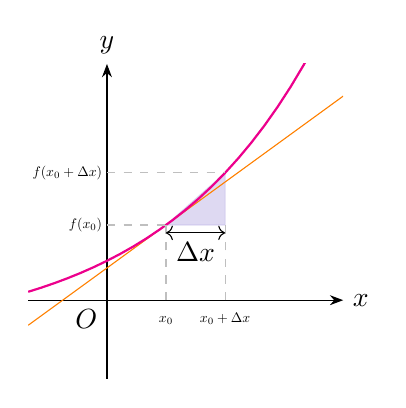
\begin{tikzpicture}
      \def\xmin{-1};
      \def\xmax{3};
      \def\ymin{-1};
      \def\ymax{3};
      \def\fn#1{exp(0.5*#1) - 0.5};
      \def\dfn#1{0.5*exp(0.5*#1)}; % \fnの導関数
      \def\xi{0.75};
      \def\xj{1.5};

      % よく使う点の座標
      \coordinate (O) at (0,0);
      \coordinate (A) at (\xi, {\fn{\xi}});
      \coordinate (B) at (\xj, {\fn{\xi}});
      \coordinate (C) at (\xj, {\fn{\xj}});
      \coordinate (D) at (A |- C);

      % 座標軸
      \draw[axis] (\xmin,0) -- (\xmax,0) node [right]{$x$};
      \draw[axis] (0,\ymin) -- (0,\ymax) node [above]{$y$};

      % 原点
      \node at (O) [below left]{$O$};

      % 傾きを表す三角形
      \draw[fill=myPurple, myPurple!80!gray, opacity=0.5] (A) --(B) -- (C) -- cycle;

      \begin{scope}
        \clip (\xmin,\ymin) rectangle (\xmax,\ymax);
        % 接線
        \draw[orange] plot[domain=\xmin:\xmax] (\x,{\fn{\xi} + \dfn{\xi}*(\x-\xi)});
        % グラフ
        \draw[magenta,thick] plot[domain=\xmin:\xmax] (\x,{\fn{\x}});
      \end{scope}

      % x軸上の目盛り
      \node (X2) at (\xj,0) [below, scale=0.5]{$\strut x_0 + \Delta x$};
      \node (X1) at (\xi,0) [below, scale=0.5, baseline = (X2.base)]{$\strut x_0$};

      % y軸上の目盛り
      \node at (0,{\fn{\xi}}) [left, scale=0.5]{$f(x_0)$};
      \node at (0,{\fn{\xj}}) [left, scale=0.5]{$f(x_0 + \Delta x)$};

      % x軸からの補助線
      \draw[auxline, thin, lightgray] (\xi,0) -- (A);
      \draw[auxline, thin, lightgray] (\xj,0) -- (B);

      % y軸からの補助線
      \draw[auxline, thin, lightgray] (0,{\fn{\xi}}) -- (A);
      \draw[auxline, thin, lightgray] (0,{\fn{\xj}}) --(C);

      % \Delta xを表す矢印
      \draw[<->] ($(A)-(0,0.1)$) -- ($(B)-(0,0.1)$) node [midway, below]{$\Delta x$};
    \end{tikzpicture}
  }
\end{center}

このとき、増分の幅$\Delta x$を狭くしていく($\Delta x$の値を小さくしていく)と、$x=x_0$付近において、関数$y=f(x)$のグラフは直線にほとんど重なるようになる。

\begin{center}
  \scalebox{2}{
    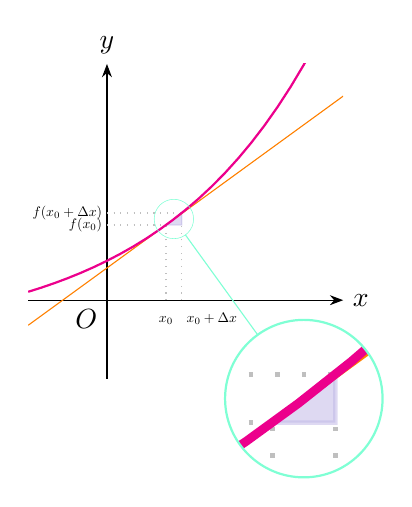
\begin{tikzpicture}[spy using outlines={circle, magnification=4, size=2cm, connect spies}]
      \def\xmin{-1};
      \def\xmax{3};
      \def\ymin{-1};
      \def\ymax{3};
      \def\fn#1{exp(0.5*#1) - 0.5};
      \def\dfn#1{0.5*exp(0.5*#1)}; % \fnの導関数
      \def\xi{0.75};
      \def\xj{0.95};

      % よく使う点の座標
      \coordinate (O) at (0,0);
      \coordinate (A) at (\xi, {\fn{\xi}});
      \coordinate (B) at (\xj, {\fn{\xi}});
      \coordinate (C) at (\xj, {\fn{\xj}});
      \coordinate (D) at (A |- C);

      % 座標軸
      \draw[axis] (\xmin,0) -- (\xmax,0) node [right]{$x$};
      \draw[axis] (0,\ymin) -- (0,\ymax) node [above]{$y$};

      % 原点
      \node at (O) [below left]{$O$};

      % x軸からの補助線
      \draw[dotted, thin, lightgray] (\xi,0) -- (A);
      \draw[dotted, thin, lightgray] (\xj,0) -- (B);
      % y軸からの補助線
      \draw[dotted, thin, lightgray] (0,{\fn{\xi}}) -- (A);
      \draw[dotted, thin, lightgray] (0,{\fn{\xj}}) --(C);

      % 傾きを表す三角形
      \draw[fill=myPurple, myPurple!80!gray, opacity=0.5] (A) --(B) -- (C) -- cycle;

      \begin{scope}
        \clip (\xmin,\ymin) rectangle (\xmax,\ymax);
        % 接線
        \draw[orange] plot[domain=\xmin:\xmax] (\x,{\fn{\xi} + \dfn{\xi}*(\x-\xi)});
        % グラフ
        \draw[magenta,thick] plot[domain=\xmin:\xmax] (\x,{\fn{\x}});
      \end{scope}

      % x軸上の目盛り
      \node (X2) at (\xj,0) [below right, scale=0.5]{$\strut x_0 + \Delta x$};
      \node (X1) at (\xi,0) [below, scale=0.5, baseline = (X2.base)]{$\strut x_0$};

      % y軸上の目盛り
      \node at (0,{\fn{\xi}}) [left, scale=0.5]{$f(x_0)$};
      \node at (0,{\fn{\xj}}) [left, scale=0.5]{$f(x_0 + \Delta x)$};

      \spy [Aquamarine] on ($(A)!.5!(C)$) in node [left] at (3.5,-1.25);
    \end{tikzpicture}
  }
\end{center}

このように、関数$f(x)$は、ある点$x_0$の付近では、

\begin{equation}
  f(x) \simeq a(x - x_0) +b
\end{equation}

という直線に近似することができる。

\vskip\baselineskip

ここで、$f(x_0)$の値を考えると、

\begin{align}
  f(x_0) & = a(x_0 - x_0) + b \\
         & = a\cdot 0 + b     \\
         & = b
\end{align}

であるから、実は$b=f(x_0)$である。

\vskip\baselineskip

一方、$a$はこの直線の傾きを表す。

そもそも、傾きとは、$x$が増加したとき、$y$がどれだけ急に(速く)増加するかを表す量である。

関数のグラフを見ると、急激に上下する箇所もあれば、なだらかに変化する箇所もある。

つまり、ある点でグラフにぴったりと沿う直線(接線)を見つけたとしても、その傾きは場所によって異なる。

そこで、「傾きは位置$x$の関数」とみなして、次のように表現しよう。

\begin{equation}
  a = f'(x)
\end{equation}

これで、先ほどの直線の式を完成させることができる。

\begin{theorem}{関数の各点の接線}
  \newline
  関数$f(x)$は、ある点$x_0$の付近では、
  \Large
  \begin{equation}
    f(x) \simeq f(x_0) + f'(x)(x - x_0)
  \end{equation}
  \normalsize
  という傾き$f'(x)$の直線に近似できる。
\end{theorem}

\subsection{接線の傾きとしての導関数}

傾きは位置$x$の関数$f'(x)$としたが、この関数がどのような関数なのか、結局傾きを計算する方法がわかっていない。

直線の傾きは$x$と$y$の増加率の比として定義されているから、まずはそれぞれの増加率を数式で表現しよう。

\begin{center}
  \scalebox{2}{
    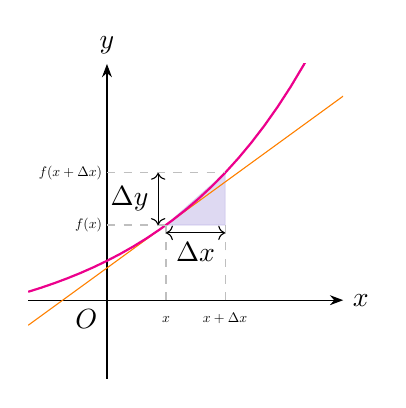
\begin{tikzpicture}
      \def\xmin{-1};
      \def\xmax{3};
      \def\ymin{-1};
      \def\ymax{3};
      \def\fn#1{exp(0.5*#1) - 0.5};
      \def\dfn#1{0.5*exp(0.5*#1)}; % \fnの導関数
      \def\xi{0.75};
      \def\xj{1.5};

      % よく使う点の座標
      \coordinate (O) at (0,0);
      \coordinate (A) at (\xi, {\fn{\xi}});
      \coordinate (B) at (\xj, {\fn{\xi}});
      \coordinate (C) at (\xj, {\fn{\xj}});
      \coordinate (D) at (A |- C);

      % 座標軸
      \draw[axis] (\xmin,0) -- (\xmax,0) node [right]{$x$};
      \draw[axis] (0,\ymin) -- (0,\ymax) node [above]{$y$};

      % 原点
      \node at (O) [below left]{$O$};

      % 傾きを表す三角形
      \draw[fill=myPurple, myPurple!80!gray, opacity=0.5] (A) --(B) -- (C) -- cycle;

      \begin{scope}
        \clip (\xmin,\ymin) rectangle (\xmax,\ymax);
        % 接線
        \draw[orange] plot[domain=\xmin:\xmax] (\x,{\fn{\xi} + \dfn{\xi}*(\x-\xi)});
        % グラフ
        \draw[magenta,thick] plot[domain=\xmin:\xmax] (\x,{\fn{\x}});
      \end{scope}

      % x軸上の目盛り
      \node (X2) at (\xj,0) [below, scale=0.5]{$\strut x + \Delta x$};
      \node (X1) at (\xi,0) [below, scale=0.5, baseline = (X2.base)]{$\strut x$};

      % y軸上の目盛り
      \node at (0,{\fn{\xi}}) [left, scale=0.5]{$f(x)$};
      \node at (0,{\fn{\xj}}) [left, scale=0.5]{$f(x + \Delta x)$};

      % x軸からの補助線
      \draw[auxline, thin, lightgray] (\xi,0) -- (A);
      \draw[auxline, thin, lightgray] (\xj,0) -- (B);

      % y軸からの補助線
      \draw[auxline, thin, lightgray] (0,{\fn{\xi}}) -- (A);
      \draw[auxline, thin, lightgray] (0,{\fn{\xj}}) --(C);

      % \Delta xを表す矢印
      \draw[<->] ($(A)-(0,0.1)$) -- ($(B)-(0,0.1)$) node [midway, below]{$\Delta x$};
      % \Delta yを表す矢印
      \draw[<->] ($(A)+(-0.1,0)$) -- ($(D)+(-0.1, 0)$) node [midway, left]{$\Delta y$};
    \end{tikzpicture}
  }
\end{center}

この図から、$y$の増加率$\Delta y$は次のように表せることがわかる。

\begin{equation}
  \Delta y = f(x + \Delta x) - f(x)
\end{equation}

この両辺を$\Delta x$で割ると、$x$の増加率$\Delta x$と$y$の増加率$\Delta y$の比率が表せる。

\begin{equation}
  \frac{\Delta y}{\Delta x} = \frac{f(x + \Delta x) - f(x)}{\Delta x}
\end{equation}

図では$\Delta x$には幅があるが、この幅を限りなく$0$に近づけると、幅というより点になる。

つまり、$\Delta x \rightarrow 0$とすれば、$\dfrac{\Delta y}{\Delta x}$は任意の点$x$での接線の傾きとなる。

「任意の点$x$での傾き」も$x$の関数であり、この関数を導関数と呼ぶ。

\begin{definition}{導関数}
  \newline
  関数$f(x)$の任意の点$x$における接線の傾き(増加の速さ)を表す関数を導関数といい、次のように定義する。
  \Large
  \begin{equation}
    f'(x) = \lim_{\Delta x \to 0} \frac{f(x + \Delta x) - f(x)}{\Delta x}
  \end{equation}
\end{definition}

\subsection{微分とその関係式}

\begin{definition}{微分}
  関数$f(x)$から、その導関数$f'(x)$を求める操作を微分という。
\end{definition}

関数のグラフから離れて、微分という「計算」を考えるにあたって、先ほどの導関数の定義式よりも都合の良い表現式がある。

$x \to 0$とした後の$\Delta x$を$dx$と書くことにして、$\displaystyle\lim_{\Delta x \to 0}$を取り払ってしまおう。

\begin{equation}
  \begin{WithArrows}
    f'(x) & = \dfrac{f(x + dx) - f(x)}{dx} \Arrow{両辺$\times dx$} \\
    f'(x)dx & = f(x + dx) - f(x) \Arrow{$f(x)$を移項} \\
    f'(x)dx + f(x) & = f(x + dx)
  \end{WithArrows}
\end{equation}

\begin{theorem}{微分の関係式}
  \Large
  \begin{equation}
    f(x + dx)= f(x) + f'(x)dx
  \end{equation}
\end{theorem}

\subsection{不連続点と微分可能性}

点$x$において連続な関数であれば、幅$\Delta x$を小さくすれば、その間の変化量$\Delta y$も小さくなるはずである。

\begin{center}
  \scalebox{2}{
    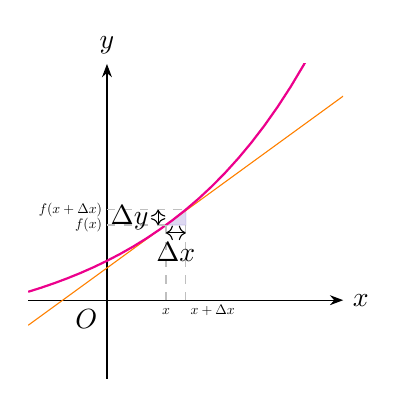
\begin{tikzpicture}
      \def\xmin{-1};
      \def\xmax{3};
      \def\ymin{-1};
      \def\ymax{3};
      \def\fn#1{exp(0.5*#1) - 0.5};
      \def\dfn#1{0.5*exp(0.5*#1)}; % \fnの導関数
      \def\xi{0.75};
      \def\xj{1};

      % よく使う点の座標
      \coordinate (O) at (0,0);
      \coordinate (A) at (\xi, {\fn{\xi}});
      \coordinate (B) at (\xj, {\fn{\xi}});
      \coordinate (C) at (\xj, {\fn{\xj}});
      \coordinate (D) at (A |- C);

      % 座標軸
      \draw[axis] (\xmin,0) -- (\xmax,0) node [right]{$x$};
      \draw[axis] (0,\ymin) -- (0,\ymax) node [above]{$y$};

      % 原点
      \node at (O) [below left]{$O$};

      % 傾きを表す三角形
      \draw[fill=myPurple, myPurple!80!gray, opacity=0.5] (A) --(B) -- (C) -- cycle;

      \begin{scope}
        \clip (\xmin,\ymin) rectangle (\xmax,\ymax);
        % 接線
        \draw[orange] plot[domain=\xmin:\xmax] (\x,{\fn{\xi} + \dfn{\xi}*(\x-\xi)});
        % グラフ
        \draw[magenta,thick] plot[domain=\xmin:\xmax] (\x,{\fn{\x}});
      \end{scope}

      % x軸上の目盛り
      \node (X2) at (\xj,0.1) [below right, scale=0.5]{$\strut x + \Delta x$};
      \node (X1) at (\xi,0.1) [below, scale=0.5, baseline = (X2.base)]{$\strut x$};

      % y軸上の目盛り
      \node at (0,{\fn{\xi}}) [left, scale=0.5]{$f(x)$};
      \node at (0,{\fn{\xj}}) [left, scale=0.5]{$f(x + \Delta x)$};

      % x軸からの補助線
      \draw[auxline, thin, lightgray] (\xi,0) -- (A);
      \draw[auxline, thin, lightgray] (\xj,0) -- (B);

      % y軸からの補助線
      \draw[auxline, thin, lightgray] (0,{\fn{\xi}}) -- (A);
      \draw[auxline, thin, lightgray] (0,{\fn{\xj}}) --(C);

      % \Delta xを表す矢印
      \draw[<->] ($(A)-(0,0.1)$) -- ($(B)-(0,0.1)$) node [midway, below]{$\Delta x$};
      % \Delta yを表す矢印
      \draw[<->] ($(A)+(-0.1,0)$) -- ($(D)+(-0.1, 0)$) node [midway, left]{$\Delta y$};
    \end{tikzpicture}
  }
\end{center}

しかし、不連続な点について考える場合は、そうはいかない。

下の図を見ると、$\Delta x$の幅を小さくしても、$\Delta y$は不連続点での関数の値の差の分までしか小さくならない。

\begin{figure}[H]
  \begin{minipage}{0.5\hsize}
    \centering
    \scalebox{1.5}{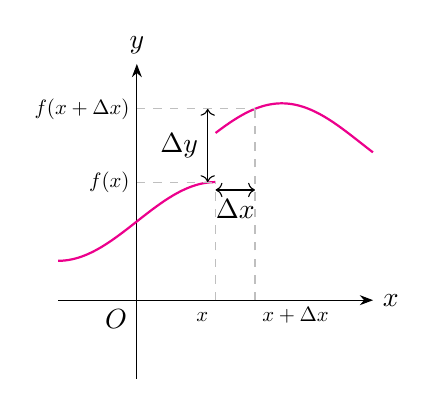
\begin{tikzpicture}
        \def\xmin{-1};
        \def\xmax{3};
        \def\ymin{-1};
        \def\ymax{3};
        \def\fnA#1{0.5*sin(deg(0.5*pi*#1))+1};
        \def\fnB#1{-0.5*cos(deg(0.5*pi*#1+0.25))+2};
        \def\xi{1};
        \def\xj{1.5};

        % よく使う点の座標
        \coordinate (O) at (0,0);
        \coordinate (A) at (\xi, {\fnA{\xi}});
        \coordinate (B) at (\xj, {\fnB{\xj}});
        \coordinate (C) at (\xj, {\fnA{\xi}});
        \coordinate (D) at (A |- B);

        % 原点
        \node at (O) [below left]{$O$};

        % 座標軸
        \draw[axis] (\xmin,0) -- (\xmax,0) node[right] {$x$};
        \draw[axis] (0,\ymin) -- (0,\ymax) node[above] {$y$};

        % 関数の描画
        \draw[domain=\xmin:\xi, samples=100, magenta,thick, smooth] plot (\x, {\fnA{\x}});
        \draw[domain=\xi:\xmax, samples=100, magenta,thick, smooth] plot (\x, {\fnB{\x}});

        % x軸上の目盛り
        \node (X2) at (\xj,0.15) [below right, scale=0.75]{$\strut x + \Delta x$};
        \node (X1) at (\xi,0.15) [below left, scale=0.75, baseline = (X2.base)]{$\strut x$};

        % y軸上の目盛り
        \node at (0,{\fnA{\xi}}) [left, scale=0.75]{$f(x)$};
        \node at (0,{\fnB{\xj}}) [left, scale=0.75]{$f(x + \Delta x)$};

        % x軸からの補助線
        \draw[auxline, thin, lightgray] (\xi,0) -- (A);
        \draw[auxline, thin, lightgray] (\xj,0) -- (B);

        % y軸からの補助線
        \draw[auxline, thin, lightgray] (0,{\fnA{\xi}}) -- (A);
        \draw[auxline, thin, lightgray] (0,{\fnB{\xj}}) --(B);

        % \Delta xを表す矢印
        \draw[<->] ($(A)-(0,0.1)$) -- ($(C)-(0,0.1)$) node [midway, below]{$\Delta x$};
        % \Delta yを表す矢印
        \draw[<->] ($(A)+(-0.1,0)$) -- ($(D)+(-0.1, 0)$) node [midway, left]{$\Delta y$};
      \end{tikzpicture}
    }
  \end{minipage}%
  \begin{minipage}{0.5\hsize}
    \centering
    \scalebox{1.5}{
      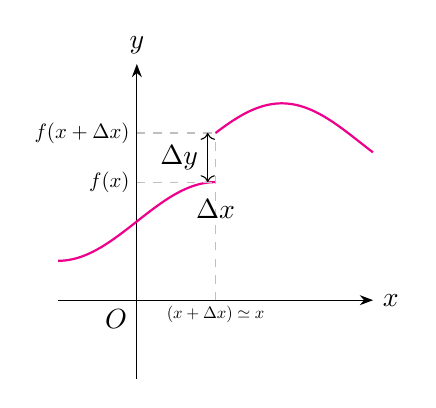
\begin{tikzpicture}
        \def\xmin{-1};
        \def\xmax{3};
        \def\ymin{-1};
        \def\ymax{3};
        \def\fnA#1{0.5*sin(deg(0.5*pi*#1))+1};
        \def\fnB#1{-0.5*cos(deg(0.5*pi*#1+0.25))+2};
        \def\xi{1};
        \def\xj{1};

        % よく使う点の座標
        \coordinate (O) at (0,0);
        \coordinate (A) at (\xi, {\fnA{\xi}});
        \coordinate (B) at (\xj, {\fnB{\xj}});
        \coordinate (C) at (\xj, {\fnA{\xi}});
        \coordinate (D) at (A |- B);

        % 原点
        \node at (O) [below left]{$O$};

        % 座標軸
        \draw[axis] (\xmin,0) -- (\xmax,0) node[right] {$x$};
        \draw[axis] (0,\ymin) -- (0,\ymax) node[above] {$y$};

        % 関数の描画
        \draw[domain=\xmin:\xi, samples=100, magenta,thick, smooth] plot (\x, {\fnA{\x}});
        \draw[domain=\xi:\xmax, samples=100, magenta,thick, smooth] plot (\x, {\fnB{\x}});

        % x軸上の目盛り
        \node (X2) at (\xj,0) [below, scale=0.6]{$ (x+ \Delta x) \simeq x$};

        % y軸上の目盛り
        \node at (0,{\fnA{\xi}}) [left, scale=0.75]{$f(x)$};
        \node at (0,{\fnB{\xj}}) [left, scale=0.75]{$f(x + \Delta x)$};

        % x軸からの補助線
        \draw[auxline, thin, lightgray] (\xi,0) -- (A);
        \draw[auxline, thin, lightgray] (\xj,0) -- (B);

        % y軸からの補助線
        \draw[auxline, thin, lightgray] (0,{\fnA{\xi}}) -- (A);
        \draw[auxline, thin, lightgray] (0,{\fnB{\xj}}) --(B);

        % \Delta xを表す矢印
        \draw ($(A)-(0,0.1)$) -- ($(C)-(0,0.1)$) node [midway, below]{$\Delta x$};
        % \Delta yを表す矢印
        \draw[<->] ($(A)+(-0.1,0)$) -- ($(D)+(-0.1, 0)$) node [midway, left]{$\Delta y$};
      \end{tikzpicture}
    }
  \end{minipage}
\end{figure}

このような不連続点においては、どんなに拡大しても、関数のグラフが直線にぴったりと重なることはない。

「拡大すれば直線に近似できる」というのが微分の考え方だが、不連続点ではこの考え方を適用できないのだ。

\vskip\baselineskip

関数の不連続点においては、微分という計算を考えることがそもそもできない。

ある点での関数のグラフが直線に重なる(微分可能である)ためには、$\Delta x \to 0$としたときに$\Delta y \to 0$となる必要がある。

\subsection{導関数のさまざまな記法}

微分を考えるときは、$\Delta x \to 0$としたときに$\Delta y \to 0$となる前提のもとで議論する。

$\Delta x$を$x \to 0$としたものを$dx$、同様に$\Delta y$を$y \to 0$としたものを$dy$とすると、ある点$x$での接線の傾きは、次のようにも表現できる。

\begin{equation}
  \frac{dy}{dx} = \lim_{\Delta x \to 0} \frac{\Delta y}{\Delta x}
\end{equation}

この接線の傾きが$x$の関数であることを表現したいときは、次のように書くこともある。

\begin{equation}
  \dfrac{dy}{dx}(x)
\end{equation}

これも一つの導関数(位置に応じた接線の傾きを表す関数)の表記法である。

この記法は、どの変数で微分しているかがわかりやすいという利点がある。

\begin{definition}{導関数のライプニッツ記法}
  \newline
  次のような記号はいずれも、関数$y = f(x)$の導関数を表す。
  \Large
  \begin{equation}
    \frac{dy}{dx} = \dfrac{dy}{dx}(x) = \dfrac{df}{dx} = \dfrac{d}{dx}f(x)
  \end{equation}
\end{definition}

特に、$\dfrac{d}{dx}f(x)$という記法は、$\dfrac{d}{dx}$の部分を微分操作を表す演算子として捉えて、「関数$f(x)$に微分という操作を施した」ことを表現しているように見える。

\begin{definition}{微分演算子}
  \newline
  関数を微分するという操作を表現する演算子を微分演算子という。\\
  例えば、次のような記号で表される。
  \Large
  \begin{equation}
    \dfrac{d}{dx}
  \end{equation}
\end{definition}

ところで、これまで使ってきた$f'(x)$という導関数の記法にも、名前がついている。

\begin{definition}{導関数のニュートン記法}
  \newline
  次の記号は、関数$y = f(x)$の導関数を表す。
  \Large
  \begin{equation}
    f'(x)
  \end{equation}
\end{definition}

この記法は、「$f$という関数から導出された関数が$f'$である」ことを表現している。

導関数はあくまでも関数$f$から派生したものであるから、$f$という文字はそのまま、加工されたことを表すために$'$をつけたものと解釈できる。

\subsection{三角関数の微分}

\begin{center}
  \scalebox{2}{
    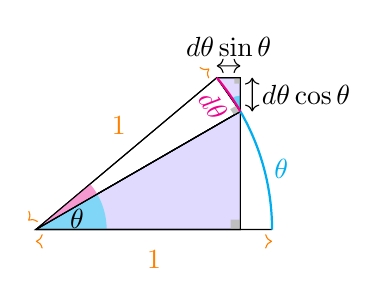
\begin{tikzpicture}[scale=3]
      \coordinate (A) at (1,0);
      \coordinate (O) at (0,0);
      \coordinate (C1) at (30:1cm);
      \coordinate (C2) at (40:1cm);
      \coordinate (H) at (C1 |- O);
      % Hのx座標とC2のy座標を持つ点
      \coordinate (H2) at (C2 -| H);

      % OとAを結ぶ線
      \draw (O) -- (A);
      % OとC1を結ぶ線
      \draw (O) -- (C1);
      % OとC2を結ぶ線
      \draw (O) -- (C2);

      % 三角形O-H-C1
      \draw[fill=myPurple, opacity=0.6] (O) -- (H) -- (C1) -- cycle;
      % 三角形C1-H-C2
      \draw[fill=myPurple, opacity=0.6] (C2) -- (H2) -- (C1) -- cycle;

      % 角A-O-C1を表す扇形
      \draw (A) -- (O) -- (C1) pic [fill=cyan!50, angle radius=9mm, "$\theta$"] {angle = A--O--C1};
      % 角C1-O-C2を表す扇形
      \draw (C1) -- (O) -- (C2) pic [fill=magenta!40, angle radius=9mm] {angle = C1--O--C2};
      % 角C1-H-C2を表す扇形
      \draw (H2) -- (C1) -- (C2) pic [fill=cyan!60, angle radius=2mm] {angle = H2--C1--C2};

      % 直角O-H-C1
      \draw (O) -- (H) -- (C1) pic [fill=lightgray, angle radius=1.25mm] {right angle = O--H--C1};
      % 直角O-C1-C2
      \draw (O) -- (C1) --(C2) pic [fill=lightgray, angle radius=0.9mm] {right angle = O--C1--C2};
      % 直角C1-H2-C2
      \draw (C1) -- (H2) -- (C2) pic [fill=lightgray, angle radius=0.75mm] {right angle = C1--H2--C2};

      % AからC1を結ぶ円弧
      \draw[cyan, thick] (A) arc (0:30:1cm) node [midway, above, right] {$\theta$};
      % C1からC2を結ぶ円弧
      \draw[magenta, thick] (C1) arc (30:40:1cm) node [midway,sloped, below] {$d\theta$};

      % C1からH2の高さを表すベクトル
      \draw[<->] ($(C1)+ (0.05, 0)$) -- ($(H2)+(0.05,0)$) node [midway, right] {$d\theta\cos \theta$};
      % C2からH2の幅を表すベクトル
      \draw[<->] ($(C2)+ (0, 0.05)$) -- ($(H2)+(0,0.05)$) node [midway, above] {$d\theta\sin \theta$};

      % OからC2の長さを表すベクトル
      \draw [<->, orange] to ($(O)!0.05!90:(C2)$) -- ($(C2)!-0.05!90:(O)$) node [midway, above, orange] { $1$ };
      % OからAの長さを表すベクトル
      \draw [<->, orange] to ($(O)-(0,0.05)$) -- ($(A)-(0,0.05)$) node [midway, below, orange] { $1$ };

      % % sin\thetaを表すベクトル
      % \draw [<->] to ($(C1)+(0.05,0)$) -- ($(H)+(0.05,0)$) node [midway, left] { $\sin \theta$ };
      % % cos\thetaを表すベクトル
      % \draw [<->] to ($(H)-(0,0.05)$) -- ($(O)-(0,0.05)$) node [midway, below] { $\cos \theta$ };
    \end{tikzpicture}
  }
\end{center}


\chapter{複素数と複素関数}

\section{複素平面}

複素数は、実部(Real Part)と虚部(Imaginary Part)という2つの数から成る。

そのため、実部を横軸に、虚部を縦軸にとった平面を考え、1つの複素数をこの平面上の1点として表すことができる。

\begin{definition}{複素平面}
  実部を横軸、虚部を縦軸にとった平面を複素平面と呼ぶ。
\end{definition}

\begin{center}
  \begin{tikzpicture}
    \def\ang{35} % 偏角
    \def\r{3} % 半径

    % x軸の描画
    \draw [axis] (-1,0) -- (4,0) node[right] {Re};
    % y軸の描画
    \draw [axis] (0,-1) -- (0,3) node[above] {Im};

    % 原点O
    \coordinate (O) at (0,0) node[below left] {O};

    % 座標軸上の点
    \coordinate[label=below right:$a$] (X) at ({\r*cos(\ang)}, 0);
    \coordinate[label=left:$b$] (Y) at (0, {\r*sin(\ang)});

    % 複素数z
    \coordinate (Z) at ({\r*cos(\ang)}, {\r*sin(\ang)});

    % 補助線の描画
    \draw[auxline] (X) -- (Z);
    \draw[auxline] (Y) -- (Z);

    % 複素数を表す数式の描画
    \node[above right] at (Z) {$a+ib$};
  \end{tikzpicture}
\end{center}

\section{複素数の絶対値}

\begin{definition}{複素数の絶対値}
  \newline
  複素平面において、原点から複素数$z$までの距離を複素数$z$の絶対値と定義する。\\
  この距離は三平方の定理から求められ、$|z|$と表す。
  \LARGE
  \begin{equation}
    |z| \coloneqq \sqrt{x^2 + y^2}
  \end{equation}
\end{definition}

\begin{center}
  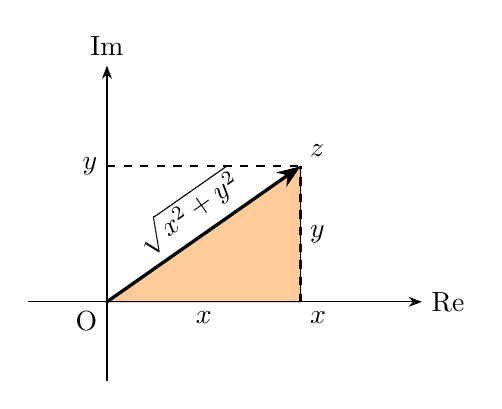
\begin{tikzpicture}
    \def\ang{35} % 偏角
    \def\r{3} % 半径

    % x軸の描画
    \draw [axis] (-1,0) -- (4,0) node[right] {Re};
    % y軸の描画
    \draw [axis] (0,-1) -- (0,3) node[above] {Im};

    % 原点O
    \coordinate (O) at (0,0) node[below left] {O};

    % 座標軸上の点
    \coordinate[label=below right:$x$] (X) at ({\r*cos(\ang)}, 0);
    \coordinate[label=left:$y$] (Y) at (0, {\r*sin(\ang)});

    % 複素数z
    \coordinate (Z) at ({\r*cos(\ang)}, {\r*sin(\ang)});

    % 三角形の描画
    \draw[fill=orange, opacity=0.4] (O) -- (X) -- (Z) -- cycle;

    % 三角形の辺のラベルの描画
    \draw (O) -- (X) node[midway, below] {$x$};
    \draw (X) -- (Z) node[midway, right] {$y$};
    \draw (O) -- (Z) node[midway, above, sloped] {$\sqrt{x^2 + y^2}$};

    % ベクトルの描画
    \draw[vector] (O) -- (Z);

    % 補助線の描画
    \draw[auxline] (X) -- (Z);
    \draw[auxline] (Y) -- (Z);

    % 複素数を表す数式の描画
    \node[above right] at (Z) {$z$};
  \end{tikzpicture}
\end{center}

\section{複素数の極形式による表現}

\begin{definition}{極形式}
  \newline
  複素数$z$は、絶対値$r$と偏角$\theta$を用いて次のように表すことができる。
  \LARGE
  \begin{equation}
    z = r(\cos\theta + i\sin\theta)
  \end{equation}
\end{definition}

\begin{center}
  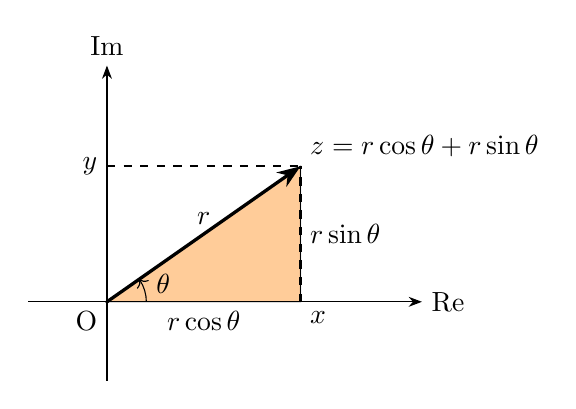
\begin{tikzpicture}
    \def\ang{35} % 偏角
    \def\r{3} % 半径

    % x軸の描画
    \draw [axis] (-1,0) -- (4,0) node[right] {Re};
    % y軸の描画
    \draw [axis] (0,-1) -- (0,3) node[above] {Im};

    % 原点O
    \coordinate (O) at (0,0) node[below left] {O};

    % 座標軸上の点
    \coordinate[label=below right:$x$] (X) at ({\r*cos(\ang)}, 0);
    \coordinate[label=left:$y$] (Y) at (0, {\r*sin(\ang)});

    % 複素数z
    \coordinate (Z) at ({\r*cos(\ang)}, {\r*sin(\ang)});

    % 三角形の描画
    \draw[fill=orange, opacity=0.4] (O) -- (X) -- (Z) -- cycle;

    % 三角形の辺のラベルの描画
    \draw (O) -- (X) node[midway, below] {$r\cos\theta$};
    \draw (X) -- (Z) node[midway, right] {$r\sin\theta$};

    % ベクトルの描画
    \draw[vector] (O) -- (Z);

    % 補助線の描画
    \draw[auxline] (X) -- (Z);
    \draw[auxline] (Y) -- (Z);

    % 偏角を表す円弧の描画
    \pic [draw, ->, "$\theta$", angle eccentricity=1.5] {angle = X--O--Z};

    % 半径を表すラベルの描画
    \draw (O) -- (Z) node[midway, above] {$r$};

    % 複素数を表す数式の描画
    \node[above right] at (Z) {$z=r\cos\theta + r\sin\theta$};
  \end{tikzpicture}
\end{center}

\section{偏角と主値}

$x=r\cos\theta$、$y=r\sin\theta$に、$r=\sqrt{x^2 + y^2}$を代入して整理した関係式から、偏角を改めて定義する。

\begin{definition}{偏角}
  \newline
  複素数$z$を極形式で表現すると、\\
  $\cos\theta=\dfrac{x}{\sqrt{x^2 + y^2}}$、$\sin\theta=\dfrac{y}{\sqrt{x^2 + y^2}}$という関係が成り立つ。\\\\
  この関係を満たす$\theta$を偏角と呼び、次のように表す。
  \LARGE
  \begin{equation}
    \arg z \coloneqq \theta
  \end{equation}
\end{definition}

ここで、$\theta$を整数回$2\pi$シフトさせても(何周回っても)、複素数$z$の値は変わらない。

つまり、1つの複素数に対して偏角の値は複数考えられるので、次のような主値を定義する。

\begin{definition}{偏角の主値}
  \newline
  $0\leq \theta \leq 2\pi$、もしくは$-\pi < \theta \leq \pi$の範囲にある偏角を偏角の主値と呼び、次のように表す。
  \LARGE
  \begin{equation}
    \Arg z \coloneqq \theta
  \end{equation}
\end{definition}

\section{共役複素数}

\begin{definition}{共役複素数}
  \newline
  複素数$z=x+iy$に対して,その共役複素数$\overline{z}$を次のように定義する。
  \LARGE
  \begin{equation}
    \overline{z}\coloneqq x-iy
  \end{equation}
\end{definition}

\begin{center}
  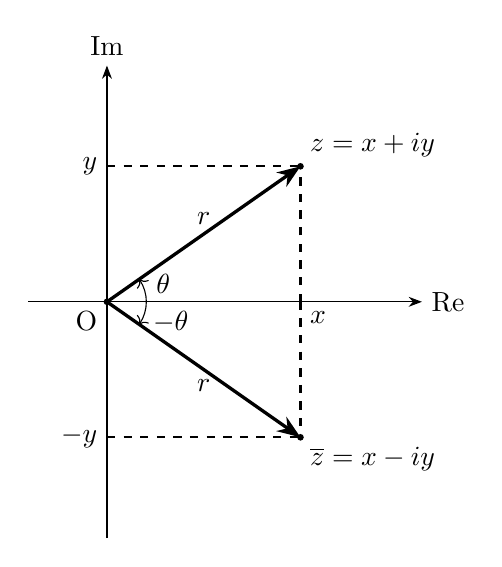
\begin{tikzpicture}
    \def\ang{35} % 偏角
    \def\r{3} % 半径

    % x軸の描画
    \draw [axis] (-1,0) -- (4,0) node[right] {Re};
    % y軸の描画
    \draw [axis] (0,-3) -- (0,3) node[above] {Im};

    % 原点O
    \coordinate (O) at (0,0) node[below left] {O};

    % 座標軸上の点
    \coordinate[label=below right:$x$] (X) at ({\r*cos(\ang)}, 0);
    \coordinate[label=left:$y$] (Y) at (0, {\r*sin(\ang)});
    \coordinate[label=left:$-y$] (-Y) at (0, {-\r*sin(\ang)});

    % 複素数z
    \coordinate (Z) at ({\r*cos(\ang)}, {\r*sin(\ang)});
    % 共役複素数z*
    \coordinate (Z*) at ({\r*cos(\ang)}, {-\r*sin(\ang)});

    % ベクトルの描画
    \draw[vector] (O) -- (Z);
    \draw[vector] (O) -- (Z*);

    % 補助線の描画
    \draw[auxline] (X) -- (Z);
    \draw[auxline] (X) -- (Z*);
    \draw[auxline] (Y) -- (Z);
    \draw[auxline] (-Y) -- (Z*);

    % 偏角を表す円弧の描画
    \pic [draw, ->, "$\theta$", angle eccentricity=1.5] {angle = X--O--Z};
    \pic [draw, <-, "$-\theta$", angle eccentricity=1.7] {angle = Z*--O--X};

    % 半径を表すラベルの描画
    \draw (O) -- (Z) node[midway, above] {$r$};
    \draw (O) -- (Z*) node[midway, below] {$r$};

    % 点の描画
    \fill (O) circle (1.2pt);
    \fill (Z) circle (1.2pt);
    \fill (Z*) circle (1.2pt);

    % 複素数を表す数式の描画
    \node[above right] at (Z) {$z=x+iy$};
    \node[below right] at (Z*) {$\overline{z}=x-iy$};
  \end{tikzpicture}
\end{center}

\begin{theorem}{共役複素数と絶対値}
  \newline
  複素数$z$とその共役複素数$\overline{z}$の積は、$z$の絶対値の二乗に等しい。
  \LARGE
  \begin{equation}
    z\overline{z} = |z|^2
  \end{equation}
\end{theorem}

\begin{proof}
  複素数$z=x+iy$とその共役複素数$\overline{z}=x-iy$の積を計算する。
  \begin{align*}
    z\overline{z} & = (x+iy)(x-iy)             \\
                  & = x^2 - ixy + ixy - i^2y^2 \\
                  & = x^2 + y^2                \\
                  & = |z|^2
  \end{align*}
\end{proof}

\section{オイラーの公式}

\begin{center}
  \def\xang{-13}
  \def\zang{45}
  \begin{tikzpicture}[x=(\xang:0.9), y=(90:0.9), z=(\zang:1.1)]
    \def\xmax{8.8}         % max x axis
    \def\ymin{-1.5}        % min y axis
    \def\ymax{1.6}         % max y axis
    \def\zmax{1.6}         % max z axis
    \def\xf{1.17*\xmax}    % x position frequency axis
    \def\A{(0.70*\ymax)}   % amplitude
    \def\T{(0.335*\xmax)}  % period
    \def\w{\zmax/11.2}     % spacing components
    \def\ang{47}           % angle
    \def\s{\ang/360*\T}    % time component
    \def\x{\A*cos(\ang)}   % real component
    \def\y{\A*sin(\ang)}   % imaginary component
    \def\N{100}            % number of samples
    \def\tick#1#2{\draw[thick] (#1) ++ (#2:0.12) --++ (#2-180:0.24)}

    % COMPLEX PLANE
    \begin{scope}[shift={(-1.6*\zmax,0,0)}]
      % 複素平面の枠
      \draw[black,fill=white,opacity=0.3,zy-plane](-1.25*\zmax,-1.25*\ymax) rectangle (1.4*\zmax,1.25*\ymax);
      % Im axis
      \draw[axis] (0,\ymin,0) -- (0,\ymax+0.02,0) node[pos=1,left=0,zy-plane] {Im};
      % Re axis
      \draw[axis] (0,0,-\zmax) -- (0,0,\zmax+0.02) node[right=1,below=0,zy-plane] {Re} coordinate (X);
      % 複素平面上の単位円
      \draw[plotline,zy-plane] (0,0) circle(0.991*\A) coordinate (O);
      % 単位円上の点P
      \fill[red,zy-plane] (\ang:{\A}) circle(0.07) coordinate(P);
      \node[blue,zy-plane,anchor=south west,scale=0.7] at (P) {$z(t)=Ae^{i\omega t}$};
      % 動径OP
      \draw[vector,thick,zy-plane] (0,0) -- (\ang:{\A-0.03}) coordinate (R);
      % 偏角を表す円弧
      \draw pic[-{>[flex'=1]},draw=blue,angle radius=14,angle eccentricity=1,"$\omega t$"{above=0,right=-0.5,yslant=0.69,scale=0.8},blue,zy-plane] {angle = X--O--R};
      % Re軸上の目盛り
      \tick{0,0,{\A}}{90};
      \tick{0,0,{-\A}}{90};
      % Im軸上の目盛り
      \tick{0,{\A},0}{\zang};
      \tick{0,{-\A},0}{\zang};
    \end{scope}

    % IMAGINARY
    \begin{scope}[shift={(0,0,1.9*\zmax)}]
      % sinを描く平面の枠
      \draw[black,fill=white,opacity=0.3,xy-plane](-0.5*\ymax,-1.2*\ymax) rectangle (1.10*\xmax,1.25*\ymax);
      % t axis
      \draw[axis] (-0.3*\ymax,0,0) -- (\xmax,0,0) node[below right,xy-plane] {$t$ [s]};
      % Im axis
      \draw[axis] (0,\ymin,0) -- (0,\ymax,0) node[left,xy-plane] {Im};
      % sin関数のグラフ
      \draw[plotline,samples=\N,smooth,variable=\t,domain=-0.05*\T:0.95*\xmax] plot(\t,{\A*sin(360/\T*\t)},0);
      % sin関数上の点I
      \fill[red,xy-plane] ({\s},{\y}) circle(0.07) coordinate(I);
      % 点Iでの波の高さを示すベクトル
      \draw[vector,thick,xy-plane] ({\s},0) --++ (0,{\y-0.03});
      \node[xy-plane,below] at ({\s},0) {$\omega t$};
      % 波の高さを表すIm軸上の目盛り
      \tick{0,{\A},0}{180};
      \tick{0,{-\A},0}{180};
      % 周期を示す目盛り
      \tick{{\T},0,0}{90} node[right=0,below,xy-plane] {\contour{white}{$T$}};
      \tick{{2*\T},0,0}{90} node[right=0,below,xy-plane] {\contour{white}{$2T$}};
      % 関数を表す数式
      \node[blue,below=0,xy-plane] at (0.4*\xmax,1.15*\ymax,0) {$y(t)=A\sin(\omega t)$};
    \end{scope}

    % REAL
    \begin{scope}[shift={(0,-1.8*\zmax,0)}]
      % cosを描く平面の枠
      \draw[black,fill=white,opacity=0.3,xz-plane] (-0.5*\ymax,-1.4*\ymax) rectangle (1.10*\xmax,1.25*\ymax);
      % t axis
      \draw[axis] (-0.3*\ymax,0,0) -- (\xmax,0,0) node[below right,xz-plane] {$t$ [s]};
      % Re axis
      \draw[axis] (0,0,-\zmax) -- (0,0,\zmax) node[left=-1,xz-plane] {Re};
      % cos関数のグラフ
      \draw[plotline,samples=\N,smooth,variable=\t,domain=-0.05*\T:0.95*\xmax] plot(\t,0,{\A*cos(360/\T*\t)});
      % cos関数上の点R
      \fill[red,xz-plane] ({\s},{\x}) circle(0.07) coordinate(R);
      % 点Rでの波の高さを示すベクトル
      \draw[vector,thick,xz-plane] ({\s},0) --++ (0,{\x-0.03});
      \node[xz-plane,below] at ({\s},0) {$\omega t$};
      % 波の高さを表すRe軸上の目盛り
      \tick{0,0,{\A}}{180};
      \tick{0,0,{-\A}}{180};
      % 周期を示す目盛り
      \tick{{\T},0,0}{\zang} node[below,xz-plane] {$T$};
      \tick{{2*\T},0,0}{\zang} node[below,xz-plane] {$2T$};
      % 関数を表す数式
      \node[blue,above=0,xz-plane] at (0.3*\xmax,-\ymax,0) {$x(t)=A\cos(\omega t)$};
    \end{scope}

    % COMPONENTS
    % 単位円上の点P、Im軸上の点I、Re軸上の点Rを結ぶ線
    \draw[red!80!black,dashed] (P) -- ({\s},{\y},{\x}) (I) -- ({\s},{\y},{\x+0.05}) ({\s},{\y-0.06},{\x}) -- (R);
    % 空間上に写したt軸
    \draw[axis,black,thick] (-0.1*\ymax,0,0) -- (\xmax,0,0) node[below right] {$t$ [s]};
    % 空間上に写したIm軸
    \draw[axis,black,thick] (0,\ymin,0) -- (0,\ymax+0.02,0) node[above] {Im};
    % 空間上に写したRe軸
    \draw[axis,black,thick] (0,0,-\zmax) -- (0,0,\zmax+0.02);
    \node[right=0.5em,below] at (0,0,\zmax+0.02) {$Re$};
    % 空間上のグラフ
    \foreach \i [evaluate={\tmin=max(-0.05*\T,(\i-0.05)*\T); \tmax=min(0.95*\xmax,(\i+1)*\T);}] in {0,...,2} {
        \draw[plotline,samples=0.4*\N,smooth,variable=\t] plot[domain=\tmin:\tmax](\t,{\A*sin(360/\T*\t)},{\A*cos(360/\T*\t)});
      }
    % 単位円上の点P、Im軸上の点I、Re軸上の点Rを結ぶ線が交わる点Z
    \fill[red] ({\s},{\y},{\x}) circle(0.07) coordinate(Z);
    % 空間上に動径OPを写したベクトル
    \draw[vector,thick] ({\s},0,0) --++ (0,{\y-0.03},{\x-0.03});
    % 周期を表すt軸上の目盛り
    \tick{{\T},0,0}{90};
    \tick{{2*\T},0,0}{90};
    % Re軸上の目盛り
    \tick{0,0,{\A}}{90};
    \tick{0,0,{-\A}}{90};
    % Im軸上の目盛り
    \tick{0,{\A},0}{\zang};
    \tick{0,{-\A},0}{\zang};
  \end{tikzpicture}
\end{center}

\chapter{フーリエ解析}

\section{波の2つの捉え方}

波は2つの捉え方ができる。

\begin{itemize}
  \item 空間的に捉える波:波の形そのもの
  \item 時間的に捉える波:波の振動
\end{itemize}

\subsection{空間的に捉える波}

波とは、一定の間隔で同じ形が繰り返されるものである。

空間的に捉える波は、まさにその波の形そのもので、波の形を位置$x$の関数として表す。

\begin{definition}{波長}
  波を構成する最小パターンの幅を波長と呼び、$\lambda$で表す。
\end{definition}

\begin{definition}{周期関数}
  次の式を満たす関数$f(x)$を、周期$\lambda$の周期関数という。
  \LARGE
  \begin{equation}
    f(x+\lambda) = f(x)
  \end{equation}
\end{definition}

\begin{definition}{波数}
  $2\pi$の長さに含まれる、波の最小パターンの数を波数という。
  \LARGE
  \begin{equation}
    k = \dfrac{2\pi}{\lambda}
  \end{equation}
\end{definition}

\subsection{時間的に捉える波}

波を時間軸から見たとき、波を構成する最小パターンは幅ではなく時間である。

その最小パターンを周期と呼ぶ。

周期は、波を時間軸から見たときの「波長」の言い換えともいえる。

\begin{definition}{周期}
  波が1回振動するのにかかる時間を周期と呼び、$T$で表す。
\end{definition}

\begin{definition}{周期関数}
  次の式を満たす関数$f(t)$を、周期$T$の周期関数という。
  \LARGE
  \begin{equation}
    f(t+T) = f(t)
  \end{equation}
\end{definition}

\begin{definition}{周波数(振動数)}
  \newline
  単位時間に含まれる、波の最小パターンの数を周波数という。
  \LARGE
  \begin{equation}
    \nu = \dfrac{1}{T}
  \end{equation}
  \normalsize
  これは、単位時間に何回振動するかを表すため、振動数とも呼ばれる。
\end{definition}

\section{角周波数と正弦波}

\begin{definition}{角周波数}
  動径が単位時間内に進む角を角周波数と呼び、$\omega$で表す。
\end{definition}

\begin{theorem}{任意の時間における動径}
  \newline
  時間が$t$だけ経過したときの動径$\theta$は、角周波数$\omega$を使って次のように表すことができる。
  \LARGE
  \begin{equation}
    \theta = \omega t
  \end{equation}
\end{theorem}

$\sin\theta$や$\cos\theta$は、$\theta=\omega t$の関係を用いると、動径$\theta$ではなく角周波数$\omega$の関数とみることができる。

\begin{definition}{正弦波}
  $\sin\omega t$や$\cos\omega t$を、角周波数$\omega$の正弦波と呼ぶ。
\end{definition}

\subsection{角周波数と振動数の関係}

円の1周は$2\pi$であり、単位時間あたりに進む円周は角周波数$\omega$である。

\footnotesize
(角周波数は「角」の大きさとして定義したが、弧度法のおかげで、「円周」の長さとしても捉えられる。)
\normalsize

ここで、単位時間あたりに進む円周$\omega$は、1周$2\pi$のうちのどれくらいだろうか?

その答えは、$\omega$を「1周あたりの量」$2\pi$で割ったものになる。

\begin{theorem}{角周波数と円周の関係}
  \newline
  角周波数$\omega$で動径が回転するとき、その動径は単位時間に
  \LARGE
  \begin{equation}
    \dfrac{\omega}{2\pi}
  \end{equation}
  \normalsize
  だけ円を回ることになる。
\end{theorem}

ここで、三角関数は円関数とも呼ばれるように、円の1周は三角関数の1振動に対応する。

振動を円周上の回転として表す三角関数のおかげで、「どれくらい回るか?」を「どれくらい振動するか?」とみることができる。

つまり、動径が単位時間に$\dfrac{\omega}{2\pi}$だけ回転するということは、単位時間に$\dfrac{\omega}{2\pi}$だけ振動するということだ。

\begin{theorem}{角周波数と振動数の関係}
  \newline
  角周波数を$\omega$とすると、振動数$\nu$は次のように表せる。
  \LARGE
  \begin{equation}
    \nu = \dfrac{\omega}{2\pi}
  \end{equation}
  \normalsize
\end{theorem}

\subsection{角周波数と周期の関係}

ここまでで、振動数$\nu$は2通りの表し方ができることがわかった。

\begin{itemize}
  \item $\nu = \dfrac{1}{T}$(周波数:単位時間に含まれる、最小波の時間幅)
  \item $\nu = \dfrac{\omega}{2\pi}$(振動数:単位時間に含まれる、振動の回数)
\end{itemize}

この2式を組み合わせて、次のような関係が得られる。

\begin{equation}
  \omega = 2\pi\nu = \dfrac{2\pi}{T}
\end{equation}

\begin{theorem}{角周波数と周期の関係}
  \newline
  角周波数を$\omega$、周期を$T$とすると、次のような関係が成り立つ。
  \LARGE
  \begin{equation}
    \omega = \dfrac{2\pi}{T}
  \end{equation}
\end{theorem}

\section{偶関数と奇関数}

$\sin$関数と$\cos$関数は、どちらも正弦波と呼ばれるが、その性質は異なる。

$\sin$は奇関数であり、$\cos$は偶関数である。

この違いが、後に議論するフーリエ級数展開においても重要な役割を果たす。

\subsection{偶関数と奇関数は異なる対称性を持つ}

\begin{definition}{偶関数}
  \newline
  グラフが$y$軸に対して対称な関数を偶関数と呼ぶ。\\
  偶関数は、任意の$x$に対して次の関係が成り立つ関数として定義される。
  \LARGE
  \begin{equation}
    f(-x) = f(x)
  \end{equation}
\end{definition}

\begin{definition}{奇関数}
  \newline
  グラフが原点に対して対称な関数を奇関数と呼ぶ。\\
  奇関数は、任意の$x$に対して次の関係が成り立つ関数として定義される。
  \LARGE
  \begin{equation}
    f(-x) = -f(x)
  \end{equation}
\end{definition}

\begin{center}
  \begin{tikzpicture}
    % 偶関数のグラフ(左側)
    \begin{scope}[xshift=-3cm]
      \clip (-2.5, -2.5) rectangle (2.5, 2.5);
      % 座標軸
      \draw[axis] (-2.5,0) -- (2.5,0) node[below] {$x$};
      \draw[axis] (0,-2) -- (0,2) node[above] {$y$};

      % 偶関数のプロット (例: y = x^2 - 1)
      \draw[thick, domain=-1.6:1.6, smooth, samples=100] plot (\x, {\x*\x - 1});

      % ラベル
      \node[below] at (0,-2) {偶関数: $f(-x) = f(x)$};
    \end{scope}

    % 奇関数のグラフ(右側)
    \begin{scope}[xshift=3cm]
      \clip (-2.5, -2.5) rectangle (2.5, 2.5);
      % 座標軸
      \draw[axis] (-2.5,0) -- (2.5,0) node[below] {$x$};
      \draw[axis] (0,-2) -- (0,2) node[above] {$y$};

      % 奇関数のプロット (例: y = x^3 - x)
      \draw[thick, domain=-1.5:1.5, smooth, samples=100] plot (\x, {\x*\x*\x - \x});

      % ラベル
      \node[below] at (0,-2) {奇関数: $f(-x) = -f(x)$};
    \end{scope}
  \end{tikzpicture}
\end{center}

1つの関数が、この両方の性質を持つことはない。

つまり、偶関数であり奇関数でもある関数は存在しない。

\subsection{積に関する性質}

\begin{theorem}{偶関数と奇関数の積}
  偶関数と奇関数の積は、奇関数となる。
\end{theorem}

\begin{proof}
  $f(x)$を奇関数、$g(x)$を偶関数とすると、
  \begin{equation}
    \begin{WithArrows}
      f(x)g(x)   & = -f(-x)g(-x) \Arrow{両辺$-1$倍して両辺入れ替え} \\
      f(-x)g(-x) & = -f(x)g(x)
    \end{WithArrows}
  \end{equation}
  となり、引数を$-1$倍すると符号が反転するため、$f(x)g(x)$は奇関数である。
\end{proof}

\begin{theorem}{奇関数どうしの積}
  奇関数と奇関数の積は、偶関数となる。
\end{theorem}

\begin{proof}
  $f(x), g(x)$を奇関数とすると、
  \begin{align}
    f(x)g(x) & = -f(-x)\cdot\{-g(-x)\} \\
             & = f(-x)g(-x)
  \end{align}
  となり、引数を$-1$倍しても符号がそのままなので、$f(x)g(x)$は偶関数である。
\end{proof}

\begin{theorem}{偶関数どうしの積}
  偶関数と偶関数の積は、偶関数となる。
\end{theorem}

\begin{proof}
  $f(x), g(x)$を偶関数とすると、
  \begin{equation}
    \begin{WithArrows}
      f(x)g(x)   & = f(-x)g(-x) \Arrow{両辺入れ替え} \\
      f(-x)g(-x) & = f(x)g(x)
    \end{WithArrows}
  \end{equation}
  となり、引数を$-1$倍しても符号がそのままなので、$f(x)g(x)$は偶関数である。
\end{proof}

\subsection{和に関する性質}

\begin{theorem}{奇関数どうしの和}
  奇関数と奇関数の和は、奇関数となる。
\end{theorem}

\begin{proof}
  $f(x), g(x)$を奇関数とすると、
  \begin{equation}
    \begin{WithArrows}
      f(x) + g(x) &= -f(-x)-g(-x) \\
      &= -\{f(-x)+g(-x)\} \Arrow{両辺$-1$倍して両辺入れ替え} \\
      f(-x) + g(x) &= -\{f(x)+g(x)\}
    \end{WithArrows}
  \end{equation}
  となり、引数を$-1$倍すると符号が反転するため、$f(x)+g(x)$は奇関数である。
\end{proof}

\begin{theorem}{偶関数どうしの和}
  偶関数と偶関数の和は、偶関数となる。
\end{theorem}

\begin{proof}
  $f(x), g(x)$を偶関数とすると、
  \begin{equation}
    f(x)+g(x) = f(-x)+g(-x)
  \end{equation}
  となり、引数を$-1$倍しても符号がそのままなので、$f(x)+g(x)$は偶関数である。
\end{proof}

\subsection{偶関数・奇関数の積分}

\begin{theorem}{偶関数の積分公式}
  \newline
  原点に関して対称な区間$-a \leq x \leq a$において、$f(x)$が偶関数なら、次の式が成り立つ。
  \LARGE
  \begin{equation}
    \int_{-a}^{a}f(x)dx = 2\int_{0}^{a}f(x)dx
  \end{equation}
\end{theorem}

\begin{center}
  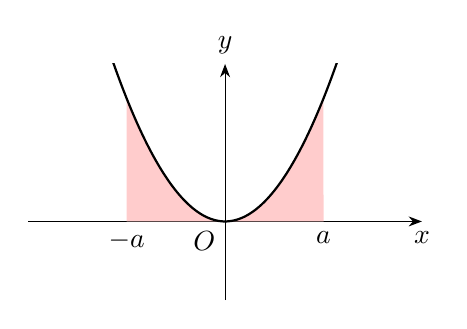
\begin{tikzpicture}
    \def\xmin{-2.5};
    \def\xmax{2.5};
    \def\ymin{-1};
    \def\ymax{2};
    \def\a{1.25};
    \def\fn#1{#1*#1}

    % 座標軸
    \draw[axis] (\xmin,0) -- (\xmax,0) node[below] {$x$};
    \draw[axis] (0,\ymin) -- (0,\ymax) node[above] {$y$};

    % x軸上の点a,-a
    \node[below] at (\a,0) {$a$};
    \node[below] at (-\a,0) {$-a$};

    % 積分が面積となる領域
    \fill [pink!80, domain=-\a:\a, variable=\x] (-\a, 0) -- plot ({\x}, {\fn{\x}}) -- (\a, 0) -- cycle;

    % 原点
    \node[below left] at (0,0) {$O$};

    % 偶関数のグラフ
    \begin{scope}
      \clip (\xmin, \ymin) rectangle (\xmax, \ymax);
      % 偶関数のプロット
      \draw[thick, domain=\xmin:\xmax, smooth, samples=100] plot (\x, {\fn{\x}});
    \end{scope}
  \end{tikzpicture}
\end{center}

\begin{theorem}{奇関数の積分公式}
  \newline
  原点に関して対称な区間$-a \leq x \leq a$において、$f(x)$が奇関数なら、次の式が成り立つ。
  \LARGE
  \begin{equation}
    \int_{-a}^{a}f(x)dx = 0
  \end{equation}
\end{theorem}

\begin{center}
  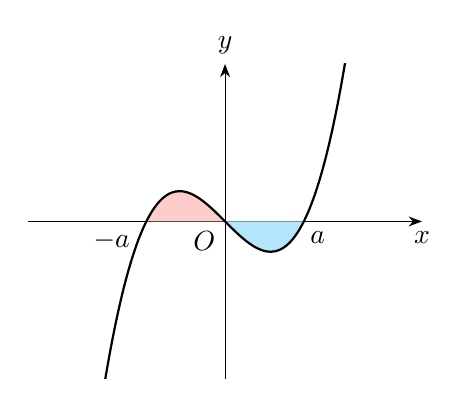
\begin{tikzpicture}
    \def\xmin{-2.5};
    \def\xmax{2.5};
    \def\ymin{-2};
    \def\ymax{2};
    \def\a{1};
    \def\fn#1{#1*#1*#1 - #1};

    % 座標軸
    \draw[axis] (\xmin,0) -- (\xmax,0) node[below] {$x$};
    \draw[axis] (0,\ymin) -- (0,\ymax) node[above] {$y$};

    % 原点
    \node[below left] at (0,0) {$O$};

    % x軸上の点a,-a
    \node[right=0.5em, below] at (\a,0) {$a$};
    \node[left=1.25em, below] at (-\a,0) {$-a$};

    % 積分が正の面積となる領域
    \fill [pink!80, domain=-\a:0, variable=\x] (-\a, 0) -- plot ({\x}, {\fn{\x}}) -- (0, 0) -- cycle;
    % 積分が負の面積となる領域
    \fill [cyan!30, domain=0:\a, variable=\x] (0, 0) -- plot ({\x}, {\fn{\x}}) -- (\a, 0) -- cycle;

    % 奇関数のグラフ
    \begin{scope}
      \clip (\xmin, \ymin) rectangle (\xmax, \ymax);
      % 奇関数のプロット
      \draw[thick, domain=\xmin:\xmax, smooth, samples=100] plot (\x, {\fn{\x}});
    \end{scope}
  \end{tikzpicture}
\end{center}

\section{フーリエ級数}

\subsection{そもそも級数とは}

\begin{definition}{級数展開}
  \newline
  ある関数$f(x)$を、より基本的な関数系
  \Large
  \begin{equation}
    \{\varphi_0(x), \varphi_1(x), \varphi_2(x), \dots\}
  \end{equation}
  \normalsize
  を使って、次のような級数で表すことを級数展開という。
  \LARGE
  \begin{equation}
    f(x) = \sum_{n=0}^{\infty} c_n \varphi_n(x)
  \end{equation}
\end{definition}

級数展開は、近似や性質の分析に役立つ。

\subsubsection{代表的な級数展開:マクローリン展開}

$f(x)$が無限回微分可能なとき、$f(x)$は多項式関数$\{x^0, x^1, x^2, \dots\}$を使って級数展開できる。

\begin{equation}
  f(x) = \sum_{n=0}^{\infty} \dfrac{f^{(n)}(0)}{n!}x^n
\end{equation}

このような級数展開をマクローリン展開という。

\subsubsection{代表的な級数展開:フーリエ級数展開}

$f(x)$が特定の条件を満たすとき、$f(x)$は三角関数を使って級数展開できる。

このような級数展開をフーリエ級数展開といい、これからの議論の対象となる。

\subsection{有限区間で定義された関数のフーリエ級数展開}

\begin{theorem}{有限区間で定義された関数のフーリエ級数展開}
  \newline
  $-\dfrac{T}{2} \leq t \leq \dfrac{T}{2}$(区間幅$T$の有限区間)で定義された関数$f(t)$について、
  \Large
  \begin{equation}
    f(t) = \labelmath{a_0 + \sum_{n=1}^{\infty} \left\{ a_n\cos\left(\dfrac{2\pi nt}{T}\right) + b_n\sin\left(\dfrac{2\pi nt}{T}\right) \right\}}{\normalsize フーリエ級数展開}
  \end{equation}
  \normalsize
  が成り立つとしたら、フーリエ係数$a_0, a_n, b_n$は次のようになる。
  \Large
  \begin{align}
    a_0 & = \dfrac{1}{T} \int_{-\frac{T}{2}}^{\frac{T}{2}} f(t) dt                                     \\
    a_n & = \dfrac{2}{T} \int_{-\frac{T}{2}}^{\frac{T}{2}} f(t) \cos\left(\dfrac{2\pi nt}{T}\right) dt \\
    b_n & = \dfrac{2}{T} \int_{-\frac{T}{2}}^{\frac{T}{2}} f(t) \sin\left(\dfrac{2\pi nt}{T}\right) dt
  \end{align}
\end{theorem}

\subsection{フーリエ級数展開の周期関数への拡張}

元の関数$f(t)$には区間の制限を設けていたが、フーリエ級数を構成する三角関数は、無限区間で定義されている。

そして、三角関数は、区間幅$T$だけずらしても同じ値をとる、周期$T$の周期関数である。

つまり、特定の区間内の関数$f(t)$の形を、無限区間内で$T$ずつずらしていっても、それを表現するフーリエ級数の式は変わらない。

関数$f(t)$が、区間の制限をなくしても同じ形を繰り返すだけ(周期関数)であれば、先ほどのフーリエ級数展開がそのまま成り立つことになる。

\begin{theorem}{周期関数のフーリエ級数展開}
  \newline
  周期$T$の周期関数$f(t)$について、
  \Large
  \begin{equation}
    f(t) = \labelmath{a_0 + \sum_{n=1}^{\infty} \left\{ a_n\cos\left(\dfrac{2\pi nt}{T}\right) + b_n\sin\left(\dfrac{2\pi nt}{T}\right) \right\}}{\normalsize フーリエ級数展開}
  \end{equation}
  \normalsize
  が成り立つとしたら、フーリエ係数$a_0, a_n, b_n$は次のようになる。
  \Large
  \begin{align}
    a_0 & = \dfrac{1}{T} \int_{-\frac{T}{2}}^{\frac{T}{2}} f(t) dt                                     \\
    a_n & = \dfrac{2}{T} \int_{-\frac{T}{2}}^{\frac{T}{2}} f(t) \cos\left(\dfrac{2\pi nt}{T}\right) dt \\
    b_n & = \dfrac{2}{T} \int_{-\frac{T}{2}}^{\frac{T}{2}} f(t) \sin\left(\dfrac{2\pi nt}{T}\right) dt
  \end{align}
\end{theorem}

\subsection{不連続点におけるフーリエ級数の値}

次のような矩形波$f(t)$では、$t=\dfrac{T}{n}$が不連続な点となる。

\begin{equation}
  f(t) = \left\{
  \begin{array}{ll}
    0 & (-\pi \leq t < 0) \\
    1 & (0 \leq t < \pi)
  \end{array}
  \right.
\end{equation}

% SQUARE WAVE
\begin{center}
  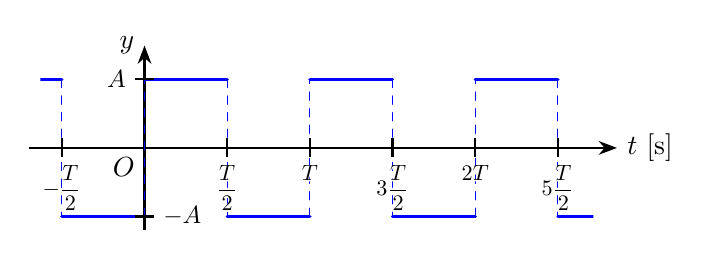
\begin{tikzpicture}
    \def\xmin{-0.7*\T}   % min x axis
    \def\xmax{6.0}       % max x axis
    \def\ymin{-1.04}     % min y axis
    \def\ymax{1.3}       % max y axis
    \def\A{0.67*\ymax}   % amplitude
    \def\T{(0.35*\xmax)} % period
    \def\f#1{\A*4/pi/(#1)*sin(360/\T*#1*Mod(\t,\T))} %Mod(360*#1*\t/\T,360)
    \def\tick#1#2{\draw[thick] (#1) ++ (#2:0.12) --++ (#2-180:0.24)}

    % AXIS
    \draw[axis,thick] (0,\ymin) -- (0,\ymax) node[left] {$y$};
    \draw[axis,thick] ({\xmin},0) -- (\xmax,0) node[below,right] {$t$ [s]};

    % PLOT
    \begin{scope}
      \clip ({0.9*\xmin},-1.1*\A) rectangle (0.95*\xmax,1.1*\A);
      \foreach \i [evaluate={\x=\i*\T/2;}] in {-2,...,5}{
          \ifodd\i
            \draw[plotline,very thick,line cap=round] (\x,{-\A}) --++ ({\T/2},0);
            \draw[plotline,dashed,thin,line cap=round]
            ({\x+\T/2},{-\A}) --++ (0,2*\A);
          \else
            \draw[plotline,very thick,line cap=round] (\x,{\A}) --++ ({\T/2},0);
            \draw[plotline,dashed,thin,line cap=round]
            ({\x+\T/2},{\A}) --++ (0,-2*\A);
          \fi
        }
    \end{scope}

    % 周期を表すラベル
    \tick{{ -\T/2},0}{90} node[below,scale=0.8] {\contour{white}{$-\dfrac{T}{2}$}};
    \tick{{  \T  },0}{90} node[below,scale=0.8] {\contour{white}{$T$}};
    \tick{{  \T/2},0}{90} node[right,below,scale=0.8] {\contour{white}{$\dfrac{T}{2}$}};
    \tick{{3*\T/2},0}{90} node[right,below,scale=0.8] {\contour{white}{$3\dfrac{T}{2}$}};
    \tick{{2*\T  },0}{90} node[right,below,scale=0.8] {\contour{white}{$2T$}};
    \tick{{5*\T/2},0}{90} node[right,below,scale=0.8] {\contour{white}{$5\dfrac{T}{2}$}};

    \tick{0,{ \A}}{  0} node[left,scale=0.9] {$A$};
    \tick{0,{-\A}}{180} node[right,scale=0.9] {$-A$};

    % 原点
    \node[below left] at (0,0) {$O$};
  \end{tikzpicture}
\end{center}

この関数をフーリエ級数展開し、$k$項までの和を求めた結果が、$s_k$のような波形となる。

% SQUARE WAVE SYNTHESIS - time domain
\begin{center}
  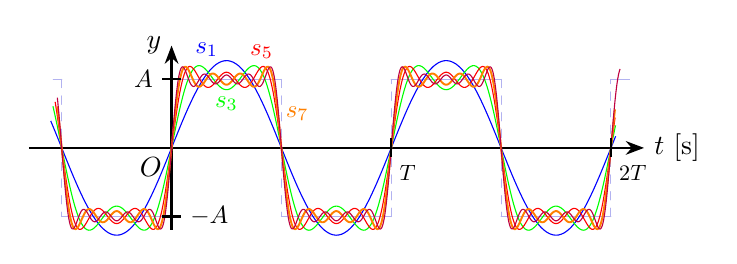
\begin{tikzpicture}
    \def\xmin{-0.65*\T}  % max x axis
    \def\xmax{6.0}       % max x axis
    \def\ymin{-1.04}     % min y axis
    \def\ymax{1.3}       % max y axis
    \def\A{0.67*\ymax}   % amplitude
    \def\f#1{\A*4/pi/(#1)*sin(360/\T*#1*Mod(\t,\T))} %Mod(360*#1*\t/\T,360)
    \def\T{(0.465*\xmax)} % period
    \def\N{100}            % number of samples
    \def\tick#1#2{\draw[thick] (#1) ++ (#2:0.12) --++ (#2-180:0.24)}

    % 元の矩形波を点線で描画
    \begin{scope}
      \clip ({-0.54*\T},-1.1*\A) rectangle (0.97*\xmax,1.1*\A);
      \foreach \i [evaluate={\x=\i*\T/2;}] in {-2,...,4}{
          \ifodd\i
            \draw[blue!80!black!30,line cap=round] (\x,{-\A}) --++ ({\T/2},0);
            \draw[blue!80!black!30,dashed,thin,line cap=round]
            ({\x+\T/2},{-\A}) --++ (0,2*\A);
          \else
            \draw[blue!80!black!30,line cap=round] (\x,{\A}) --++ ({\T/2},0);
            \draw[blue!80!black!30,dashed,thin,line cap=round]
            ({\x+\T/2},{\A}) --++ (0,-2*\A);
          \fi
        }
    \end{scope}

    % AXIS
    \draw[axis,thick] (0,\ymin) -- (0,\ymax) node[left] {$y$};
    \draw[axis,thick] ({\xmin},0) -- (\xmax,0) node[below,right] {$t$ [s]};

    % PLOT
    \draw[plotline, thin,samples=\N,smooth,variable=\t,domain=-0.55*\T:0.94*\xmax] plot(\t,{\f{1}});
    \draw[plotline, thin,green,samples=3*\N,smooth,variable=\t,domain=-0.54*\T:0.94*\xmax] plot(\t,{\f{1}+\f{3}});
    \draw[plotline, thin,red,samples=5*\N,smooth,variable=\t,domain=-0.53*\T:0.94*\xmax] plot(\t,{\f{1}+\f{3}+\f{5}});
    \draw[plotline, thin,orange,line width=0.7,samples=7*\N,smooth,variable=\t,domain=-0.52*\T:0.94*\xmax] plot(\t,{\f{1}+\f{3}+\f{5}+\f{7}});
    \draw[plotline, thin,purple,samples=9*\N,smooth,variable=\t,domain=-0.52*\T:0.95*\xmax] plot(\t,{\f{1}+\f{3}+\f{5}+\f{7}+\f{9}});

    % NUMBERS
    \node[blue,  above,scale=0.9] at ({0.16*\T},1.20*\A) {$s_1$};
    \node[green, below,scale=0.9] at ({0.25*\T},0.88*\A) {$s_3$};
    \node[red,   above,scale=0.9] at ({0.41*\T},1.17*\A) {$s_5$};
    \node[orange,right,scale=0.9] at ({0.48*\T},0.50*\A) {$s_7$};

    % 周期を表すラベル
    \tick{{  \T},0}{90} node[below right,scale=0.8] {$T$};
    \tick{{2*\T},0}{90} node[below right,scale=0.8] {$2T$};

    % 周波数を表すラベル
    \tick{0,{ \A}}{  0} node[left,scale=0.9] {$A$};
    \tick{0,{-\A}}{180} node[right,scale=0.9] {$-A$};

    % 原点
    \node[below left] at (0,0) {$O$};
  \end{tikzpicture}
\end{center}

$k$が大きくなるほど、$s_k$は元の矩形波$f(t)$に近づいていることがわかる。

ここで、元の関数の不連続点である$t=\dfrac{T}{n}$において、$s_k$は不連続点を通過している。

例えば、$t=0$において、$t=0$より左側では$-A$に近い値、右側では$A$に近い値をとる。

\begin{itemize}
  \item $t=0$に右から近づいていくと、$s_k$は$A$に近づいていく(右極限は$A$)
  \item $t=0$に左から近づいていくと、$s_k$は$-A$に近づいていく(左極限は$-A$)
\end{itemize}

そして、$t=0$において、$s_k$は$A$と$-A$の間の値(原点)を通過している。

一般に、不連続となる$t$において、フーリエ級数展開の値は、その点での左右の極限値の平均値となる。

\begin{theorem}{不連続点におけるフーリエ級数の収束}
  \newline
  $f(t)$が$t=a$で不連続のとき、フーリエ級数の値は左極限$f(a-0)$と右極限$f(a+0)$の平均値に収束する。
  \LARGE
  \begin{equation}
    \lim_{t \to a} s_k(t) = \dfrac{f(a-0) + f(a+0)}{2}
  \end{equation}
\end{theorem}

\subsection{フーリエ級数展開の意味}

フーリエ級数展開の式は、

\begin{itemize}
  \item $1$の係数が$a_0$
  \item $\cos\left(\dfrac{2\pi nt}{T}\right)$の係数が$a_n$
  \item $\sin\left(\dfrac{2\pi nt}{T}\right)$の係数が$b_n$
\end{itemize}

となっていた。

フーリエ級数展開は、次の基本関数系を使った級数展開といえる。

\begin{equation}
  \left\{1, \cos\left(\dfrac{2\pi nt}{T}\right), \sin\left(\dfrac{2\pi nt}{T}\right)\right\}
\end{equation}

ここで、

\begin{review}
  $\sin\omega t$や$\cos\omega t$は、角周波数$\omega$の正弦波と呼ばれる
\end{review}

ことを思い出すと、フーリエ級数展開を構成する基本関数系は、角周波数$\omega_n = \dfrac{2\pi n}{T}$の正弦波である。

(1は$\cos\dfrac{2\pi nt}{T}$における、$n=0$の場合だと考えることができる。)

つまり、フーリエ級数展開は、関数$f(t)$を角周波数$\omega_n$の正弦波に分解することである。

\begin{center}
  % SYNTHESIS 3D
  \begin{tikzpicture}[x=(-20:0.9), y=(90:0.9), z=(42:1.1)]
    \def\xmax{6.5}        % max x axis
    \def\ymin{-1.2}       % min y axis
    \def\ymax{1.6}        % max y axis
    \def\zmax{5.8}        % max z axis
    \def\xf{1.17*\xmax}   % x position frequency axis
    \def\A{(0.60*\ymax)}  % amplitude
    \def\T{(0.335*\xmax)} % period
    \def\w{\zmax/11.2}    % spacing components
    \def\N{100}           % number of samples
    \def\f#1{\A*4/pi/(#1)*sin(360/\T*#1*Mod(\t,\T))} %Mod(360*#1*\t/\T,360)
    \def\tick#1#2{\draw[thick] (#1) ++ (#2:0.12) --++ (#2-180:0.24)}

    % COMPONENTS
    \foreach \i/\col [evaluate={\z=\w*\i;}] in {11/cyan,9/purple,7/orange,5/red,3/green,1/blue}{
        %\draw[black!30] ({\T},0.1,\z) --++ (0,-0.2,0);
        %\draw[black!30] ({2*\T},0.1,\z) --++ (0,-0.2,0);
        % 分解された各波の座標軸
        \draw[axis,black!30] (0,0,\z) --++ (0.93*\xmax,0,0);
        % 分解された各波
        \draw[plotline,\col,opacity=0.8,thick,samples=\i*\N,smooth,variable=\t,domain=-0.05*\T:0.87*\xmax] plot(\t,{\f{\i}},\z);
      }

    % TIME DOMAIN
    \begin{scope}[shift={(0,0,-0.17*\zmax)}]
      % 時間領域を表す平面
      \draw[black,fill=white,opacity=0.3,xy-plane] (-0.1*\xmax,-1.25*\ymax) rectangle (1.13*\xmax,1.25*\ymax);
      % 横軸
      \draw[axis,thick] (-0.05*\xmax,0,0) -- (\xmax,0,0) node[below right,xy-plane] {$t$ [s]};
      % 縦軸
      \draw[axis,thick] (0,\ymin,0) -- (0,\ymax,0) node[left,xy-plane] {$y$};
      % 時間領域での関数のグラフ
      \draw[plotline,blue!90!black,very thick,samples=9*\N,smooth,variable=\t,domain=-0.05*\T:0.9*\xmax] plot(\t,{\f{1}+\f{3}+\f{5}+\f{7}+\f{9}+\f{11}},0);
      % 周期を示すラベル
      \tick{{\T},0,0}{90} node[below,scale=0.9,xy-plane] {\contour{white}{$T$}};
      \tick{{2*\T},0,0}{90} node[below,scale=0.9,xy-plane] {\contour{white}{$2T$}};
      % 平面を説明するラベル
      \node[scale=0.8,xy-plane] at (0.4*\xmax,-\ymax,0) {時間の世界(連続的)};
    \end{scope}

    % FREQUENCY DOMAIN
    \begin{scope}[shift={(\xf,0,0)}]
      % 周波数領域を表す平面
      \draw[black,fill=white,opacity=0.3,zy-plane] (-0.13*\zmax,-1.25*\ymax) rectangle (1.26*\zmax,1.25*\ymax);
      % 縦軸
      \draw[axis,thick] (0,0.8*\ymin,0) -- (0,\ymax,0) node[above=2,left=0,zy-plane] {$b_n$};
      % 横軸
      \draw[axis,thick] (0,0,-0.05*\zmax) --++ (0,0,1.13*\zmax) node[below right=-1,zy-plane] {$f_n$ $\left[\frac{1}{\mathrm{s}}\right]$};
      % 平面を説明するラベル
      \node[scale=0.8,zy-plane] at (0,-\ymax,0.65*\zmax) {周波数の世界(離散的)};
      % 周波数領域での関数のグラフ
      \draw[blue!30,dashed,samples=3*\N,smooth,variable=\t,domain=0.074*\zmax:1.02*\zmax] plot(0,{\A*4/pi/\t*\w},\t);
      % 各周波数成分
      \foreach \i/\col [evaluate={\z=\w*\i;}] in {11/cyan,9/purple,7/orange,5/red,3/green,1/blue}{
          % 周波数成分の高さを示す補助線
          \draw[\col,dash pattern=on 2 off 2] (0,0,\z) --++ (0,{\A*4/pi/\i},0);
          % 周波数成分の値を示す点
          \fill[\col,canvas is zy plane at x=0] (\z,{\A*4/pi/\i}) circle(0.07);
          % 横軸上の目盛りとそのラベル
          \tick{0,0,\z}{90} node[below,scale=0.85,zy-plane]{$\dfrac{\i}{T}$};
          % 横軸上の各目盛りの中点
          \foreach \i [evaluate={\z=\w*\i;}] in {2,4,...,10}{
              \fill[blue!60!black,zy-plane] (\z,0) circle(0.07);
            }
        }
    \end{scope}
  \end{tikzpicture}
\end{center}

関数$f(t)$がどのような周波数成分で構成されているか?を解き明かすのがフーリエ級数展開で、フーリエ係数は時間領域から周波数領域へのマッピングの役割を果たしている。

\subsection{フーリエ級数展開のさまざまな表現式}

フーリエ級数展開の式は、文献によって異なるいくつかの形で表現される。

\subsubsection{定数項をまとめた表現}

定数項$a_0$を、$a_n$の$n=0$の場合として考えることができる。

その場合、フーリエ級数展開は次のように表される。

\begin{theorem}{フーリエ級数展開(フーリエ係数を整理した表現)}
  \newline
  周期$T$の周期関数$f(t)$について、
  \Large
  \begin{equation}
    f(t) = \labelmath{\dfrac{a_0}{2} + \sum_{n=1}^{\infty} \left\{ a_n\cos\left(\dfrac{2\pi nt}{T}\right) + b_n\sin\left(\dfrac{2\pi nt}{T}\right) \right\}}{\normalsize フーリエ級数展開}
  \end{equation}
  \normalsize
  が成り立つとしたら、フーリエ係数$a_n, b_n$は次のようになる。
  \Large
  \begin{align}
    a_n & = \dfrac{2}{T} \int_{-\frac{T}{2}}^{\frac{T}{2}} f(t) \cos\left(\dfrac{2\pi nt}{T}\right) dt \\
    b_n & = \dfrac{2}{T} \int_{-\frac{T}{2}}^{\frac{T}{2}} f(t) \sin\left(\dfrac{2\pi nt}{T}\right) dt
  \end{align}
\end{theorem}

\subsubsection{角周波数を使った表現}

角周波数$\omega_0=\dfrac{2\pi}{T}$を使って、フーリエ級数展開の式を書き換えることもできる。

\begin{theorem}{フーリエ級数展開(角周波数を使った表現)}
  \newline
  周期$T$の周期関数$f(t)$について、角周波数$\omega_0$を用いて、
  \Large
  \begin{equation}
    f(t) = \labelmath{a_0 + \sum_{n=1}^{\infty} \left( a_n\cos \omega_0 nt + b_n\sin \omega_0 nt \right)}{\normalsize フーリエ級数展開}
  \end{equation}
  \normalsize
  が成り立つとしたら、フーリエ係数$a_0, a_n, b_n$は次のようになる。
  \Large
  \begin{align}
    a_0 & = \dfrac{1}{T} \int_{-\frac{T}{2}}^{\frac{T}{2}} f(t) dt                 \\
    a_n & = \dfrac{2}{T} \int_{-\frac{T}{2}}^{\frac{T}{2}} f(t) \cos\omega_0 nt dt \\
    b_n & = \dfrac{2}{T} \int_{-\frac{T}{2}}^{\frac{T}{2}} f(t) \sin\omega_0 nt dt
  \end{align}
\end{theorem}

\subsubsection{区間を0始まりにずらした表現}

有限区間$-\dfrac{T}{2} \leq t \leq \dfrac{T}{2}$で定義された関数のフーリエ級数展開を考えてきたが、その有限区間は区間幅が$T$であればなんでもよい。

特に、$0 \leq t \leq T$で定義された関数のフーリエ級数展開を考えることも多い。

区間を変えても、周期関数への拡張は同様の議論により成り立ち、次のことがいえる。

\begin{theorem}{フーリエ級数展開(積分区間を0始まりにした表現)}
  \newline
  周期$T$の周期関数$f(t)$について、
  \Large
  \begin{equation}
    f(t) = \labelmath{a_0 + \sum_{n=1}^{\infty} \left\{ a_n\cos\left(\dfrac{2\pi nt}{T}\right) + b_n\sin\left(\dfrac{2\pi nt}{T}\right) \right\}}{\normalsize フーリエ級数展開}
  \end{equation}
  \normalsize
  が成り立つとしたら、フーリエ係数$a_0, a_n, b_n$は次のようになる。
  \Large
  \begin{align}
    a_0 & = \dfrac{1}{T} \int_{0}^{T} f(t) dt                                     \\
    a_n & = \dfrac{2}{T} \int_{0}^{T} f(t) \cos\left(\dfrac{2\pi nt}{T}\right) dt \\
    b_n & = \dfrac{2}{T} \int_{0}^{T} f(t) \sin\left(\dfrac{2\pi nt}{T}\right) dt
  \end{align}
\end{theorem}

このフーリエ係数の式は、区間$-\dfrac{T}{2} \leq t \leq \dfrac{T}{2}$の場合の式を平行移動+置換積分することで示される。

\subsection{奇関数のフーリエ級数(フーリエ正弦級数)}

$f(t)$が奇関数の場合、それを表現するフーリエ級数には、奇関数しか入らない。

奇関数と奇関数の和が奇関数になることから、そう予想できる。

偶関数$\cos$の項が消え、奇関数$\sin$の項だけが残ることを確かめるため、各フーリエ係数を計算してみよう。

\subsubsection{定数項$a_0$}

原点に対して対称な範囲での奇関数の積分は$0$になるから、

\begin{align}
  a_0 & = \dfrac{1}{T} \int_{-\frac{T}{2}}^{\frac{T}{2}} \oddFn{f(t)} dt \\
      & = 0
\end{align}

\subsubsection{$\cos$の項の係数$a_n$}

$\int$の中身を見ると、奇関数と偶関数の積は奇関数になるので、積分結果は$0$になる。

\begin{align}
  a_n & = \dfrac{2}{T} \int_{-\frac{T}{2}}^{\frac{T}{2}} \oddFn[0.4]{\oddFn{f(t)} \evenFn{\cos\left(\dfrac{2\pi nt}{T}\right)}} dt \\
      & = 0
\end{align}

\subsubsection{$\sin$の項の係数$b_n$}

$\int$の中身を見ると、奇関数と奇関数の積は偶関数になるので、

\begin{review}
  偶関数の積分公式
  \begin{equation}
    \int_{-a}^{a}f(x)dx = 2\int_{0}^{a}f(x)dx
  \end{equation}
\end{review}

を使って計算する。

\begin{align}
  b_n & = \dfrac{2}{T} \int_{-\frac{T}{2}}^{\frac{T}{2}} \evenFn[0.4]{\oddFn{f(t)} \oddFn{\sin\left(\dfrac{2\pi nt}{T}\right)}} dt \\
      & = \dfrac{2}{T} \cdot 2 \int_{0}^{\frac{T}{2}} f(t) \sin\left(\dfrac{2\pi nt}{T}\right) dt                                  \\
      & = \dfrac{4}{T} \int_{0}^{\frac{T}{2}} f(t) \sin\left(\dfrac{2\pi nt}{T}\right) dt
\end{align}

\subsubsection{まとめ:フーリエ正弦級数}

以上より、$a_0$、$a_n$は$0$になるため、奇関数のフーリエ級数は、$\sin$の項だけで表現される。

奇関数のフーリエ級数は、フーリエ正弦級数と呼ばれる。
\begin{theorem}{フーリエ正弦級数}
  \newline
  周期$T$の周期関数$f(t)$が奇関数であり、
  \Large
  \begin{equation}
    f(t) = \labelmath{\sum_{n=1}^{\infty} b_n\sin\left(\dfrac{2\pi nt}{T}\right)}{\normalsize フーリエ正弦級数}
  \end{equation}
  \normalsize
  が成り立つとしたら、フーリエ係数$b_n$は次のようになる。
  \Large
  \begin{align}
    b_n & = \dfrac{4}{T} \int_{0}^{\frac{T}{2}} f(t) \sin\left(\dfrac{2\pi nt}{T}\right) dt
  \end{align}
\end{theorem}

\subsection{偶関数のフーリエ級数(フーリエ余弦級数)}

$f(t)$が偶関数の場合、それを表現するフーリエ級数には、偶関数しか入らない。

偶関数と偶関数の和が偶関数になることから、そう予想できる。

奇関数$\sin$の項が消え、偶関数$\cos$の項だけが残ることを確かめるため、各フーリエ係数を計算してみよう。

\subsubsection{定数項$a_0$}

偶関数の積分公式を使って計算する。

\begin{align}
  a_0 & = \dfrac{1}{T} \int_{-\frac{T}{2}}^{\frac{T}{2}} \evenFn{f(t)} dt \\
      & = \dfrac{1}{T} \cdot 2 \int_{0}^{\frac{T}{2}} f(t) dt             \\
      & = \dfrac{2}{T} \int_{0}^{\frac{T}{2}} f(t) dt
\end{align}

\subsubsection{$\cos$の項の係数$a_n$}

$\int$の中身を見ると、偶関数と偶関数の積は偶関数になるので、偶関数の積分公式を使って計算する。

\begin{align}
  b_n & = \dfrac{2}{T} \int_{-\frac{T}{2}}^{\frac{T}{2}} \evenFn[0.3]{\evenFn{f(t)} \evenFn{\cos\left(\dfrac{2\pi nt}{T}\right)}} dt \\
      & = \dfrac{2}{T} \cdot 2 \int_{0}^{\frac{T}{2}} f(t) \cos\left(\dfrac{2\pi nt}{T}\right) dt                                    \\
      & = \dfrac{4}{T} \int_{0}^{\frac{T}{2}} f(t) \cos\left(\dfrac{2\pi nt}{T}\right) dt
\end{align}

\subsubsection{$\sin$の項の係数$b_n$}

$\int$の中身を見ると、偶関数と奇関数の積は奇関数になるので、積分結果は$0$になる。

\begin{align}
  b_n & = \dfrac{2}{T} \int_{-\frac{T}{2}}^{\frac{T}{2}} \oddFn[0.4]{\evenFn{f(t)} \oddFn{\sin\left(\dfrac{2\pi nt}{T}\right)}} dt \\
      & = 0
\end{align}

\subsubsection{まとめ:フーリエ余弦級数}

以上より、$b_n$は$0$になるため、偶関数のフーリエ級数は、$\cos$の項だけで表現される。

偶関数のフーリエ級数は、フーリエ余弦級数と呼ばれる。

\begin{theorem}{フーリエ余弦級数}
  \newline
  周期$T$の周期関数$f(t)$が偶関数であり、
  \Large
  \begin{equation}
    f(t) = a_0 + \labelmath{\sum_{n=1}^{\infty} a_n\cos\left(\dfrac{2\pi nt}{T}\right)}{\normalsize フーリエ余弦級数}
  \end{equation}
  \normalsize
  が成り立つとしたら、フーリエ係数$a_0, a_n$は次のようになる。
  \Large
  \begin{align}
    a_0 & = \dfrac{2}{T} \int_{0}^{\frac{T}{2}} f(t) dt                                     \\
    a_n & = \dfrac{4}{T} \int_{0}^{\frac{T}{2}} f(t) \cos\left(\dfrac{2\pi nt}{T}\right) dt
  \end{align}
\end{theorem}

\chapter{線形システム}

\section{線形性}

\begin{definition}{線形性の1つの解釈}
  システムにおいて、次のような性質を線形性という。
  \begin{enumerate}
    \item 倍の刺激があれば、倍の反応が生まれる
    \item 2つの刺激があれば、それぞれが独立して反応する
  \end{enumerate}
\end{definition}

\end{document}
